\documentclass{beamer}
\usepackage[utf8]{inputenc}

\usetheme{Madrid}
\usecolortheme{default}
\usepackage{amsmath,amssymb,amsfonts,amsthm}
\usepackage{txfonts}
\usepackage{tkz-euclide}
\usepackage{listings}
\usepackage{adjustbox}
\usepackage{array}
\usepackage{tabularx}
\usepackage{gvv}
\usepackage{lmodern}
\usepackage{circuitikz}
\usepackage{tikz}
\usepackage{graphicx}
\usepackage{caption}
\captionsetup{labelformat=empty}  % removes "Figure:"


\setbeamertemplate{page number in head/foot}[totalframenumber]

\usepackage{tcolorbox}
\tcbuselibrary{minted,breakable,xparse,skins}



\definecolor{bg}{gray}{0.95}
\DeclareTCBListing{mintedbox}{O{}m!O{}}{%
	breakable=true,
	listing engine=minted,
	listing only,
	minted language=#2,
	minted style=default,
	minted options={%
		linenos,
		gobble=0,
		breaklines=true,
		breakafter=,,
		fontsize=\small,
		numbersep=8pt,
		#1},
	boxsep=0pt,
	left skip=0pt,
	right skip=0pt,
	left=25pt,
	right=0pt,
	top=3pt,
	bottom=3pt,
	arc=5pt,
	leftrule=0pt,
	rightrule=0pt,
	bottomrule=2pt,
	toprule=2pt,
	colback=bg,
	colframe=orange!70,
	enhanced,
	overlay={%
		\begin{tcbclipinterior}
			\fill[orange!20!white] (frame.south west) rectangle ([xshift=20pt]frame.north west);
	\end{tcbclipinterior}},
	#3,
}
\lstset{
	language=C,
	basicstyle=\ttfamily\small,
	keywordstyle=\color{blue},
	stringstyle=\color{orange},
	commentstyle=\color{green!60!black},
	numbers=left,
	numberstyle=\tiny\color{gray},
	breaklines=true,
	showstringspaces=false,
}
\begin{document}

\title 
{1.5.32}
\date{August 29,2025}

\author 
{Navya Priya - EE25BTECH11045}
\graphicspath{./figs}


\frame{\titlepage}
\begin{frame}{Question}
 Find the ratio in which the line segment joining the points $(1,−3)$ and $(4,5)$ is divided
 by X axis.
\end{frame}

\begin{frame}{Equation}
Let $\vec{A}$ = \myvec{1\\-3}, $\vec{B}$ = \myvec{$x$\\0} and $\vec{C}$ = \myvec{4\\5}\\

As the points $\vec{A,B,C}$ are collinear
The matrix 
\begin{align*}
\myvec{ \vec{B}-\vec{A} & \vec{C}-\vec{A} }^\top
\textt{has \, rank \, 1.}
\end{align*}

\textbf{Equation Used:}
\begin{align*}
    \Vec{B}=\frac{\Vec{A}+k\Vec{C}}{1+k}
\end{align*}

\end{frame}

\begin{frame}{Theoretical Solution}
\begin{align}
\myvec{ \vec{B}-\vec{A} & \vec{C}-\vec{A} }^\top = \myvec{3&x-1\\8&3}^\top
\end{align}
\begin{align}
\myvec{ \vec{B}-\vec{A} & \vec{C}-\vec{A} }^\top = \myvec{3&8\\x-1&3}
\end{align}
\begin{align}
\myvec{3&8\\x-1&3}&\xlongleftrightarrow{R_{2}\rightarrow8R_{2}-3R_{1}} \myvec{3&8\\8(x-1)-9&0}
\end{align}
\begin{align}
\implies\xleftrightarrow{R_{1}\rightarrow\frac{R_{1}}{3}}\myvec{1&\frac{8}{3}\\8x-17&0}
\end{align}

\end{frame}
\begin{frame}{Theoretical solution}
\begin{align}
\implies\xleftrightarrow{R_{2}\rightarrow R_{2}-\brak{8x-17}R_{1}}\myvec{1&\frac{8}{3}\\[3pt]0&\frac{8\brak{17-8x}}{3}}
\end{align}

 To satisfy collinearity condition, the rank of above matrix should be 1. Hence,
\begin{align}
\frac{8\brak{17-8x}}{3} = 0
\end{align}

\begin{align}
    x = 17/8
\end{align}
\end{frame}

\begin{frame}{Ratio}
Assume the ratio $\vec{B}$ divides $\vec{A}$  and $\vec{C}$ be k:1
\begin{align}
    k = \frac{\myvec{\vec{A} - \vec{B}}^\top \myvec{\vec{B} - \vec{C}}}{\norm{\myvec{\vec{B} - \vec{C}}}^2}
\end{align}
After substituting the values of $\vec{A},\, \vec{B} \, and \, \vec{C}$
\begin{align}
    k = \frac{1095}{1825}
\end{align}
\begin{align}
    k = \frac{3}{5}
\end{align}
\centering
\begin{large}Hence the ratio is 3:5.\end{large}
\end{frame}

\begin{frame}[fragile]{C code}
\begin{lstlisting}
#include <stdio.h>
// Structure for a 2D point/vector

typedef struct {
    double x;
    double y;
} Point;

// Function to apply section formula

Point sectionFormula(Point A, Point B, double m, double n) {
   Point P;
     P.x = (m * B.x + n * A.x) / (m + n);
     P.y = (m * B.y + n * A.y) / (m + n);
    return P;
}
\end{lstlisting}
\end{frame}

\begin{frame}[fragile]{Call C.py}
\begin{lstlisting}
import ctypes

# Load the shared library
ratio_lib = ctypes.CDLL("./ratio.so")   # use "ratio.dll" on Windows

# Declare function argument & return types
ratio_lib.find_ratio.argtypes = [ctypes.c_double, ctypes.c_double,
                                 ctypes.c_double, ctypes.c_double]
ratio_lib.find_ratio.restype = ctypes.c_double

# Points (1, -3) and (4, 5)
x1, y1 = 1, -3
x2, y2 = 4, 5

# Call C function
ratio = ratio_lib.find_ratio(x1, y1, x2, y2)

print(f"The ratio in which the X-axis divides the line segment is {ratio:.2f} : 1")
\end{lstlisting}
\end{frame}

\begin{frame}[fragile]{plot.py}
\begin{lstlisting}
import matplotlib.pyplot as plt
import numpy as np

# Points
A = (1, -3)
B = (17/8, 0)
C = (4, 5)

# Plot points
plt.figure(figsize=(6,6))
plt.scatter(*A, color="red", label="A(1, -3)")
plt.scatter(*B, color="blue", label="B(17/8, 0)")
plt.scatter(*C, color="green", label="C(4, 5)")

# Connect points with lines
x_vals = [A[0], B[0], C[0], A[0]]
y_vals = [A[1], B[1], C[1], A[1]]
plt.plot(x_vals, y_vals, linestyle="--", color="black")


\end{lstlisting}
\end{frame}

\begin{frame}[fragile]{plot.py}
\begin{lstlisting}

# Add text labels at coordinates
plt.text(A[0]+0.1, A[1]-0.3, "A(1, -3)", fontsize=10, color="red")
plt.text(B[0]+0.1, B[1]-0.3, "B(17/8, 0)", fontsize=10, color="blue")
plt.text(C[0]+0.1, C[1]+0.3, "C(4, 5)", fontsize=10, color="green")

# Labels and grid
plt.xlabel("x-axis")
plt.ylabel("y-axis")
plt.axhline(0, color="black", linewidth=0.5)
plt.axvline(0, color="black", linewidth=0.5)
plt.grid(True, linestyle="--", alpha=0.6)
plt.legend()
plt.title("Triangle ABC with Coordinates")

plt.show()

\end{lstlisting}
\end{frame}

\begin{frame}{Plot}
    \begin{figure}
        \centering
        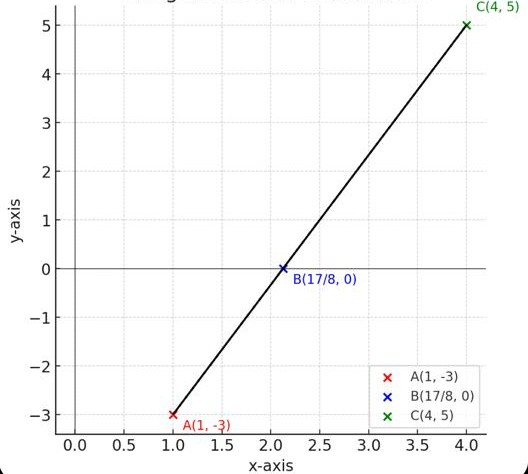
\includegraphics[width=0.5\columnwidth]{figs/graph.png}
        \caption{Plot of Intersection of AB by X-axis}
        \label{fig:graph.png}
    \end{figure}
\end{frame}


\end{document}